\section{Exploraci??n Univariada}\label{univariada}

En esta secci??n exploro cada ??ndice. En esta secci??n exploro cada ??ndice. En esta secci??n exploro cada ??ndice. En esta secci??n exploro cada ??ndice. En esta secci??n exploro cada ??ndice. En esta secci??n exploro cada ??ndice. En esta secci??n exploro cada ??ndice. En esta secci??n exploro cada ??ndice. En esta secci??n exploro cada ??ndice.





Para conocer el comportamiento de las variables se ha preparado la Tabla \ref{Tfrecuencias}, donde se describe la distribuci??n de las modalidades de cada variable. Los n??meros representan la situaci??n de algun pa??s en ese indicador, donde el mayor valor num??rico es la mejor situaci??n.

% latex table generated in R 3.5.0 by xtable 1.8-2 package
% Fri Jun 29 16:15:32 2018
\begingroup\normalsize
\begin{longtable}{llrrr}
\caption{Tablas de Frecuencia de la variables en estudio} \\ 
 \textbf{Variable} & \textbf{Levels} & $\mathbf{n}$ & $\mathbf{\%}$ & $\mathbf{\sum \%}$ \\ 
  \hline \hline
WorldFreedom & 1 & 55 & 26.7 & 26.7 \\ 
   & 3 & 62 & 30.1 & 56.8 \\ 
   & 5 & 89 & 43.2 & 100.0 \\ 
   \hline
 & all & 206 & 100.0 &  \\ 
   \hline
\hline
EconomicFreedom & 1 & 21 & 10.1 & 10.1 \\ 
   & 2 & 78 & 37.7 & 47.8 \\ 
   & 3 & 74 & 35.8 & 83.6 \\ 
   & 4 & 28 & 13.5 & 97.1 \\ 
   & 5 & 6 & 2.9 & 100.0 \\ 
   \hline
 & all & 207 & 100.0 &  \\ 
   \hline
\hline
PressFreedom & 1 & 22 & 10.7 & 10.7 \\ 
   & 2 & 53 & 25.7 & 36.4 \\ 
   & 3 & 66 & 32.0 & 68.5 \\ 
   & 4 & 48 & 23.3 & 91.8 \\ 
   & 5 & 17 & 8.2 & 100.0 \\ 
   \hline
 & all & 206 & 100.0 &  \\ 
   \hline
\hline
Democracy & 1 & 60 & 29.1 & 29.1 \\ 
   & 2 & 45 & 21.8 & 51.0 \\ 
   & 4 & 82 & 39.8 & 90.8 \\ 
   & 5 & 19 & 9.2 & 100.0 \\ 
   \hline
 & all & 206 & 100.0 &  \\ 
   \hline
\hline
\hline
\label{Tfrecuencias}
\end{longtable}
\endgroup

Como apreciamos en la Tabla \ref{Tfrecuencias}, los pa??ses en la mejor situaci??n son los menos, salvo en el caso del \emph{??ndice de libertas mundial}\footnote{N??tese que esto se puede deber a la {\bf menor} cantidad de categor??as.}

\clearpage

Para resaltar lo anterior, tenemos la Figura \ref{barplots} en la p??gina \pageref{barplots}. 


%%%%% figure
\begin{figure}[h]
\centering
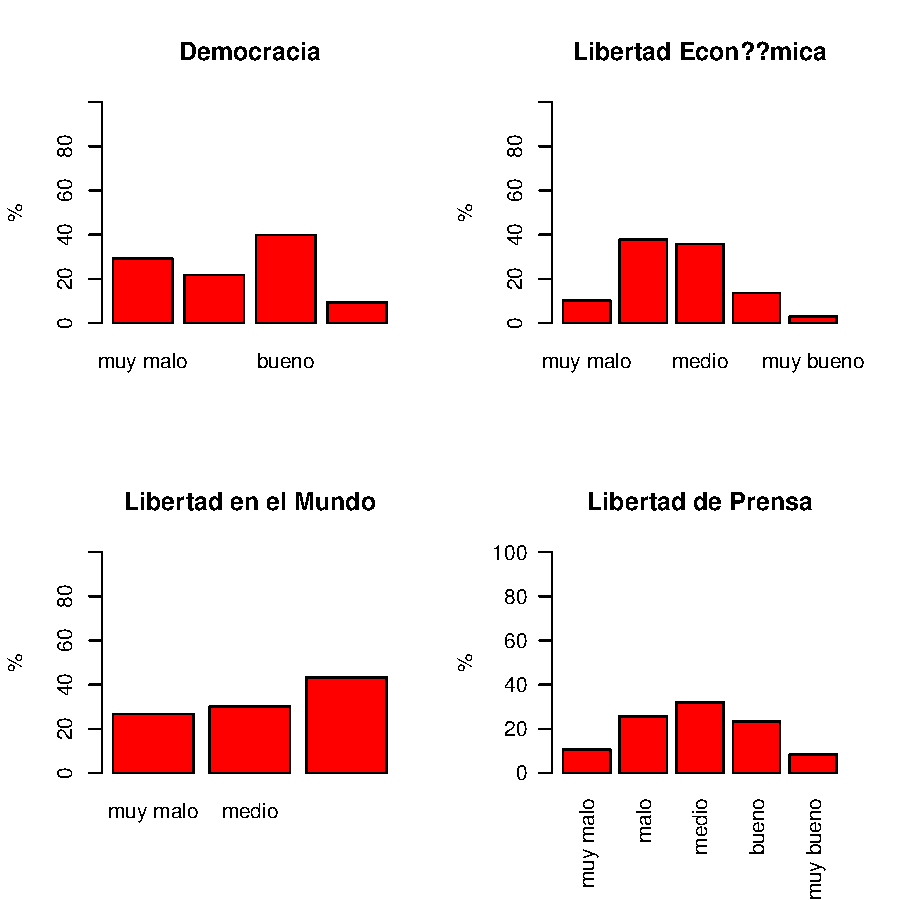
\includegraphics{paperVersion_7_univariada-barplots}
\caption{Distribuci??n de Indicadores}
\label{barplots}
\end{figure}

Adem??s de la distribuci??n de los variable, es importante saber el valor central. Como los valores son de naturaleza ordinal debemos pedir la {\bf mediana} y otras medidas de posici??n (como los \emph{cuartiles}, los que no pediremos pues son pocos valores). La mediana de cada variable la mostramos en la Tabla \ref{stats} en la p??gina \pageref{stats}.

% Table created by stargazer v.5.2.2 by Marek Hlavac, Harvard University. E-mail: hlavac at fas.harvard.edu
% Date and time: Fri, Jun 29, 2018 - 16:15:33
\begin{table}[!htbp] \centering 
  \caption{Medidas estad??sticas} 
  \label{stats} 
\begin{tabular}{@{\extracolsep{5pt}}lcc} 
\\[-1.8ex]\hline 
\hline \\[-1.8ex] 
Statistic & \multicolumn{1}{c}{N} & \multicolumn{1}{c}{Median} \\ 
\hline \\[-1.8ex] 
WorldFreedom & 206 & 3.000 \\ 
EconomicFreedom & 207 & 3 \\ 
PressFreedom & 206 & 3.000 \\ 
Democracy & 206 & 2.000 \\ 
\hline \\[-1.8ex] 
\end{tabular} 
\end{table} 




\endinput
